%%%%%%%%%%%%%%%%%%%%%%%%%%%%%%%%%%%%%%%%%%%%%%%%%%%%%%%%%%%%%%%%%%%%%%%%%%%%%%%%
% file:    talk.Rnw
% authors: Peter DeWitt, peter.dewitt@ucdenver.edu %
% Talk to be given at the HPC Launch for Rosalind at UCD.
%
% This file is based on a template made avialble by
% Copyright 2007 by Marco Barisione
% Copyright 2011 by Henricus Bouwmeester
%
% This file may be distributed and/or modified
%
% 1. under the LaTeX Project Public License and/or
% 2. under the GNU Public License.
%%%%%%%%%%%%%%%%%%%%%%%%%%%%%%%%%%%%%%%%%%%%%%%%%%%%%%%%%%%%%%%%%%%%%%%%%%%%%%%%
\documentclass[10pt]{beamer}
%\usefonttheme{serif}
\usepackage[T1]{fontenc}
\usepackage{etex}

%%%%%%%%%%%%%%%%%%%%%%%%%%%%%%%%%%%%%%%%%%%%%%%%%%%%%%%%%%%%%%%%%%%%%%%%%%%%%%%%
% Set up the ucdDenver theme
\newif\ifuseblack
% for black theme, this should be
%     \useblacktrue
% for the white theme, this should be
%     \useblackfalse
\useblacktrue

\usetheme[pageofpages=of,                    % String used between the current page and the
                                             % total page count.
          bullet=circle,                     % Use circles instead of squares for bullets.
          titleline=true,                    % Show a line below the frame title.
          showdate=true,                     % show the date on the title page
          alternativetitlepage=true,         % Use the fancy title page.
          titlepagelogo=./figure/CUAnschutz_c_clr, % Logo for the first page.
          % Logo for the header on first page.
          \ifuseblack
             headerlogo=./figure/pubHealth_tt2_rgb_rv_tp.pdf,
          \else
             headerlogo=./figure/csph_biostatistics-v2.pdf,    % Logo for white background.
          \fi
          watermark=./figure/csph_biostatistics-v2,               % Watermark used in every page.
          watermarkheight=50pt,              % Height of the watermark.
          watermarkheightmult=6,             % The watermark image is 6 times bigger
                                             % than watermarkheight.
          ]{UCDenver}

\ifuseblack
   \usecolortheme{ucdblack}
\else
   \usecolortheme{ucdwhite}
\fi

%%%%%%%%%%%%%%%%%%%%%%%%%%%%%%%%%%%%%%%%%%%%%%%%%%%%%%%%%%%%%%%%%%%%%%%%%%%%%%%%
% Title Page Setup
\author[Peter~E.~DeWitt]{Peter~E.~DeWitt, M.S., Ph.D. Candidate\\{peter.dewitt@ucdenver.edu}\vspace{0.25in}}
\title[]{Statistical Methods Research:\\Running Simulations with R in a High Performance
Computing Environment}
\institute[CSPH, UCD, BIOS]{Colorado School of Public Health\\University of Colorado Denver\\Department of Biostatistics and Informatics}
\date{14 Feburary 2017}
 
%%%%%%%%%%%%%%%%%%%%%%%%%%%%%%%%%%%%%%%%%%%%%%%%%%%%%%%%%%%%%%%%%%%%%%%%%%%%%%%%
\begin{document} 
\watermarkoff

\begin{frame}[t,plain]
  \titlepage
\end{frame}

\begin{frame}
  \frametitle{My Project}
  \begin{itemize}
    \item Working towards a Ph.D. in Biostatistics
    \item[]
    \item Explain the interaction between day-of-cycle, age, and time-to-menopause
      observed in the changes to reproductive hormone profiles expressed during
      the menopausal transition.
    \item[]
    \item Aim 1: Parsimonious B-Spline Regression Model via Control Polygon
      Reduction (CPR)
    \item[]
    \item I've developed a novel method selection approach for enumeration and
      placement of knots for B-splines.  
  \end{itemize}
\end{frame}

\begin{frame}
  \frametitle{Why I Needed A HPC}
  \begin{itemize}
    \item Simulations to show how CPR compares to
      \begin{itemize}
        \item A standard likelihood-based forward-step model selection approach,
        \item A standard likelihood-based backward-step model selection approach,
        \item P-splines
      \end{itemize}

    \item[]

    \item Start with $L$ internal knots:
      \begin{itemize}
        \item CPR requires $L + 1$ regression fits,
        \item Forward-step requires $L + 1$ regression fits,
        \item Backward-step requires $L(L+1)/2 + 1$ regression fits,
        \item P-splines requires $L + 1$ regression fits.
      \end{itemize}

    \item[]

      % 3 * (80 + 1) + 80*81/2 + 1
    \item For $L = 80$ a total of 3,484 regression models to fit.
      
  \end{itemize}
\end{frame}

\begin{frame}
  \frametitle{Why I Needed A HPC}
  \begin{itemize}
    \item Simulations:
      \begin{itemize}
        \item Four functions.
        \item Modeling under ordinary least squares and under mixed effect models.
        \item Differing sample sizes, model, and subject specific errors.
      \end{itemize}
    \item[]
    \item 144 sets of initial conditions.
    \item[]
      % 144 * 1000 * (3484)
    \item $501,696,000$ total regression models to fit.

    \item[]

    \item As a beta user I used:
      \begin{itemize}
        \item 176,742 core hours
        \item \$0.116 per core hour = \$20,502.07
      \end{itemize}
  \end{itemize}
\end{frame}

\begin{frame}
  \frametitle{My HPC Pipeline}
  \framesubtitle{Hardware, Software, RAM, and Disk Usage}
  \begin{itemize}
    \item Hardware
      \begin{itemize}
        \item A lot of computation cores
      \end{itemize}

    \item Software
      \begin{itemize}
        \item SLURM
        \item R
        \item tar
      \end{itemize}

    \item RAM
      \begin{itemize}
        \item Low enough that the 4GB per core was default sufficient.
      \end{itemize}

    \item Disk Space
      \begin{itemize}
        \item Less than 2 GB, tarballs total 633 MB.
        \item A lot of small files where generated.
        \item Originally only had 50,000 inode limit on {\tt \$HOME} and
          {\tt \$SCRATCH}, extended to 100,000 inode limit.
      \end{itemize}
  \end{itemize} 
\end{frame}

\begin{frame}
  \frametitle{Difficulties}
  \begin{itemize}
    \item Number of Files.
      \begin{itemize} 
        \item Solution: generate a controlled number of files and place into a
          tarball for each set of initial conditions.
      \end{itemize}

    \item[]

    \item Getting a Job to run to completion.
      \begin{itemize}
        \item Option 1: Request lots of nodes and cores.
          \begin{itemize}
            \item Use GNU parallel to manage the run.
            \item Did not work well for me.
            \item Queue time for resources was high.
            \item Getting a good estimate for the time required to run the sim
              was difficult. (More on this later.)
            \item[]
          \end{itemize}
        \item Option 2: Use SLURM Arrays to request a few resources many times.
          \begin{itemize}
            \item This worked well for me.
            \item Less queue time.
            \item Leaves more resource open for others.
          \end{itemize}
      \end{itemize}
  \end{itemize}
\end{frame}

\begin{frame}
  \frametitle{Estimating Time Need For An Iteration}
  \small
  \vspace{-0.2in}
  \begin{itemize}
    \item Differences between my desktop and Rosalind
      \begin{tabular}{p{0.75in}ll}
            & Rosalind                                  & My Desktop \\ \hline
        OS  & Red Hat Enterprise 7.2                    & Debian 8.7 (jessie) \\
        CPU & Intel(R) Xeon(R) E5-2680 v3 & Intel(R) Core(TM) i7-3770 \\
        Speed & 2.50GHz & 3.40GHz \\ \hline
      \end{tabular} 

    \item I have configured my desktop to use OpenBLAS for linear algebra.
    \item[]
    \item QR Decompositions is the biggest time consuming part of my work.
    \item[]
    \item Benchmarking on desktop was not helpful.
    \item[]
    \item My one wish for Rosalind: A Testing QOS.
  \end{itemize}
\end{frame}

\begin{frame}[fragile]
  \frametitle{My Workflow}
  \begin{itemize}
    \item Three types of files
      \begin{enumerate}
        \item R scripts for generating one data set and running the sim.
        \item bash script for submitting a job
        \item bash script for submitting all jobs.
      \end{enumerate}
    \item[]
    \item Examples follow.
  \end{itemize}
\end{frame}

\begin{frame}[fragile]
  \frametitle{Example R Script}
  \small
  \vspace{-0.2in}
  \begin{verbatim}
# file: doppler-lmer-sim.R
# 
# Five input args 
# s obs_per_subject sigma_alpha sigma_epsilon outdir

inparams <- commandArgs(trailingOnly = TRUE)

# Build a data set
# ....

# Run the sim
# ....

# Save results 
# ....
\end{verbatim}
\end{frame}

\begin{frame}[fragile]
  \frametitle{Example Job Submission File}
  \scriptsize
  \vspace{-0.2in}
\begin{verbatim}
#!/bin/bash
# file: doppler-lmer-sruns.sh

#SBATCH --nodes 1
#SBATCH --ntasks-per-node=20
#SBATCH --cpus-per-task=1 

if [ $# -ne 5 ]; then
  echo "expected five arguments"
  exit 1
fi

module load R

mkdir -p $5
mkdir -p $5/results
mkdir -p $5/timers
mkdir -p $5/logs

Rscript --vanilla doppler-lme4-sim.R $1 $2 $3 $4 $5 > \
  $5/logs/log.${SLURM_ARRAY_JOB_ID}_${SLURM_ARRAY_TASK_ID} &
# ... omitted lines ...
Rscript --vanilla doppler-lme4-sim.R $1 $2 $3 $4 $5 > \
  $5/logs/log.${SLURM_ARRAY_JOB_ID}_${SLURM_ARRAY_TASK_ID} &
wait
\end{verbatim}
\end{frame}

\begin{frame}[fragile]
  \frametitle{Example Submit all Jobs}
  \small
\begin{verbatim}
#!/bin/bash

# submitjobs.sh

sbatch --array=1-50 --time=01:00:00 --job-name=d2a \
  doppler-lme4-sruns.sh 2   100 0.1 0.1 dop2-sa01-se01-n0100

sbatch --array=1-50 --time=02:00:00 --job-name=d2b \
  doppler-lme4-sruns.sh 2   500 0.1 0.1 dop2-sa01-se01-n0500

sbatch --array=1-50 --time=04:00:00 --job-name=d2c \
  doppler-lme4-sruns.sh 2  1000 0.1 0.1 dop2-sa01-se01-n1000

# ... omitted lots of rows ...
# ... omitted lots of rows ...

\end{verbatim}
\end{frame}

\begin{frame}
  \frametitle{Interesting Results}
  \begin{columns}
    \begin{column}{0.6\linewidth}
  \begin{itemize}
    \item Control Polygon Reduction vs.\ other model selection tools:
      \begin{itemize}
        \item Faster,
        \item Regression models with as good, or better fits, on a
          degree-of-freedom for degree-of-freedom comparison.
      \end{itemize}
    \item[]
    \item Want to know more: 
      \begin{itemize}
        \item Dissertation defense April 10.
        \item Control Polygon Reduction,
        \item Control Net Reduction,
        \item Software, and
        \item Clinical inference.
      \end{itemize}
  \end{itemize} 
\end{column}
\begin{column}{0.4\linewidth}
  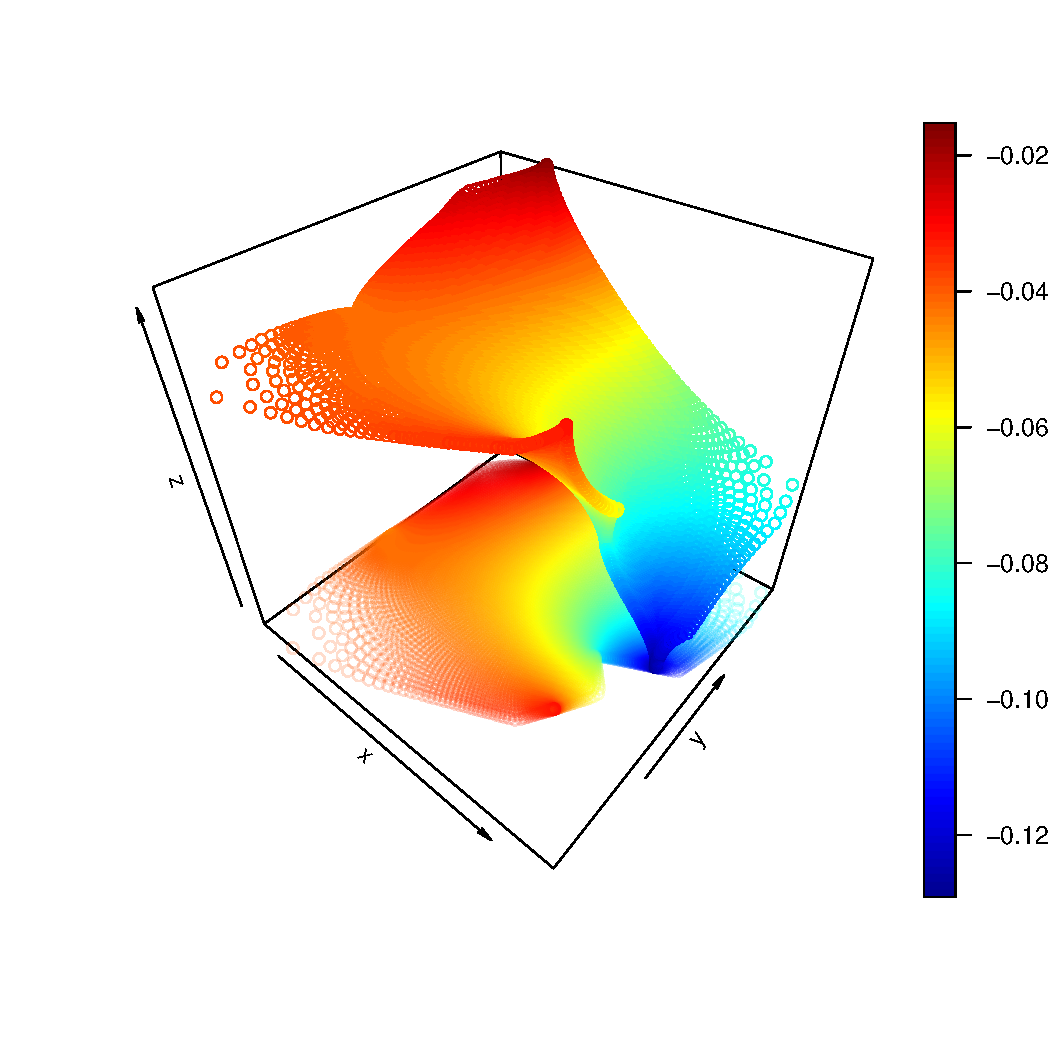
\includegraphics[width=\textwidth]{Rplots}
\end{column}
\end{columns}
\end{frame}

\begin{frame}
  \frametitle{Wish List}
  \begin{itemize}
    \item A Testing QOS
      \begin{itemize}
        \item At least two Nodes.
        \item Low wall time.
        \item High priority use.
      \end{itemize}
    \item[]
    \item Add to the "Getting Started" document
      \begin{itemize}
        \item Limits on storage, size and quantity.
        \item Details on queueing priority.
      \end{itemize}
    \item[]
    \item Community site to hosting examples, Q\&A.
    \item[]
    \item Configuration and Testing to minimize cost.
      \begin{itemize}
        \item 20 parallel jobs, one core each, or
        \item 10 parallel jobs, two cores each, or
        \item 5 parallel jobs, four cores each?
      \end{itemize}
  \end{itemize}
\end{frame}
\end{document}
%%%%%%%%%%%%%%%%%%%%%%%%%%%%%%%%%%%%%%%%%%%%%%%%%%%%%%%%%%%%%%%%%%%%%%%%%%%%%%%%
% End of file
%%%%%%%%%%%%%%%%%%%%%%%%%%%%%%%%%%%%%%%%%%%%%%%%%%%%%%%%%%%%%%%%%%%%%%%%%%%%%%%%
